\documentclass{article}
\usepackage{tikz}
\usetikzlibrary{patterns,decorations.pathmorphing,positioning, shapes.multipart, calc,arrows, shapes.geometric}
\usepackage[dvipsnames]{xcolor}

\begin{document}
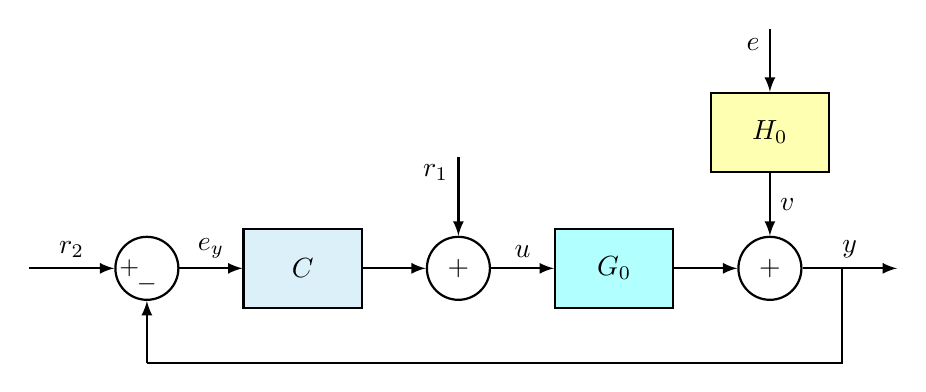
\begin{tikzpicture}[circ/.style = {draw, circle, minimum size=8mm, inner sep=0pt}, thick ]

%--- Nodes ---
% sum_r2
\node[circ]  (sum_r2) at (0,   0) {};
\node[left=-1pt] at (sum_r2.center){\small $+$};
\node[below=-1pt] at (sum_r2.center){\small $-$};

% C
\node[draw, fill=SkyBlue!30, minimum width=15mm, minimum height=10mm, right=8mm of sum_r2 ] (C) {$C$};

% sum_r1
\node[circ , right=8mm of C ]  (sum_r1) {$+$};

% G0
\node[draw, fill=Cyan!30, minimum width=15mm, minimum height=10mm , right=8mm of sum_r1 ] (G0)    {$G_0$};

% sum_v
\node[circ, , right=8mm of G0 ]  (sum_v) {$+$};

% H0
\node[draw, fill=Yellow!30, minimum width=15mm, minimum height=10mm, above=8mm of sum_v ] (H0)  {$H_0$};

%--- Input r2 ---
\draw[-latex] (-1.5, 0) -- node[above]{$r_2$} (sum_r2);

%--- sum_r2 -> C -> sum_r1 ---
\draw[-latex] (sum_r2) -- node[above]{$e_y$} (C);
\draw[-latex] (C) -- (sum_r1);

%--- r1 drops into sum_r1 from above ---
\draw[-latex] ([yshift=10mm]sum_r1.north) node[left ,yshift=-2mm]{$r_1$} -- (sum_r1);

%--- sum_r1 -> G0 ---
\draw[-latex] (sum_r1) -- node[above]{$u$} (G0);

%--- G0 -> sum_v ---
\draw[-latex] (G0) -- (sum_v);

%--- e -> H0 -> v -> sum_v ---
\draw[-latex] ([yshift=8mm]H0.north) node[left,yshift=-2mm]{$e$} -- (H0);
\draw[-latex] (H0) -- node[right]{$v$} (sum_v);

%--- sum_v -> y output ---
\draw[-latex] (sum_v) -- node[above]{$y$} ([xshift=12mm] sum_v.east);

%--- Feedback: y branches back to sum_r2 bottom ---
\coordinate (ybranch) at ([xshift=5mm] sum_v.east);
\draw (ybranch) --+(0, -1.2) -- (0, -1.2);
\draw[-latex] (0, -1.2) -- (sum_r2.south);

\end{tikzpicture}
\end{document}
